\section{Discussion}
\subsection{Performance of ZIVA}
Dimensionality reduction is an essential step for downstream analysis such as clustering and trajectory inference. In this study, we proposed a new model for reducing the dimensionality of single cell sequencing data: zero-inflated variational autoencoder (ZIVA) based on the model in VASC. We added a dropout model and its parameter fitting process and adjusted the network structure and loss function (adjusted reconstruction error and added nuclear norm). We tested the performance of ZIVA on several datasets and compared it with six other methods. The result shows that ZIVA can achieve better results in some cases especially for lineage data. 

Some popular methods such as tSNE focus on the local structure but cannot preserve global structure well. It can greatly separate the clusters of the cells but may fails when data are continuous distributed. Some methods try to keep global structure by maximize the explainable variations but fail to preserve subtle local structures such as PCA. ZIVA have a good balance between local structure and global structure. The result shows that ZIVA can recover the subtle batch effects and can also well recover the cell developmental lineages.

A shortcoming of ZIVA is the relatively long running time. For the large datasets that contains thousands of cells, ZIVA may cost several hours on a desktop-level computer. It would be better if we can compress the model to reduce the time costing.

Variational autoencoder is a great framework with high expansibility. Except from optimizing ZIVA model, we are also trying two other possible application. The first is deep clustering. By simultaneously performing dimensionality reduction and clustering, it is possible to get better performance on both tasks. The second is the graph variational autoencoder model. It performs the dimensionality reduction by constructing the graph structure in high dimensional space and preserving it to two dimensions. These two works are still in progress.

\subsection{Deep clustering for scRNA-seq data}
Because of the high dimensionality and high sparsity of the single cell sequencing data, conventional clustering methods usually have poor performance on high dimensional data. Therefore, scRNA-seq data needs to be presented in a lower dimensional space by reducing the dimensionality to enable the clustering process. The traditional pipelines usually perform dimensionality reduction and clustering as separate parts \cite{wu2020tools}. However, some researches recently shows that performing dimensionality reduction and clustering jointly can achieve better results of both clustering and dimensionality reduction \cite{yang2017towards}. For example, some researchers use Gussian mixture model to cluster images when performing variational autoencoder to reduce the dimensionality of those images \cite{prasad2020variational}. Such methods that uses deep learning to aid clustering tasks are called deep clustering.

For scRNA-seq data, we can also perform deep clustering to improve the performance of clustering and dimensionality reduction. Because there are usually several cell types in a scRNA-seq dataset, in the latent space, those cell types should fall into clusters naturally. For scRNA-seq analysis, we hope to distinguish those clusters by dimensionality reduction and clustering. In this case, we can perform deep clustering methods to cluster cells and reduce the dimensionality of data at the same time. By doing so, we can not only get nice clustering results but also get a great visualization result that have greatly separated clusters that enable us to identify cell sub-populations clearly \cite{tian2019clustering}. 

We performed deep clustering by applying the clustering algorithms to the two dimensional latent variables of variational autoencoder. The basic structure are as Figure \ref{dcstru}. 

\begin{figure}[htb!]
    \centering
    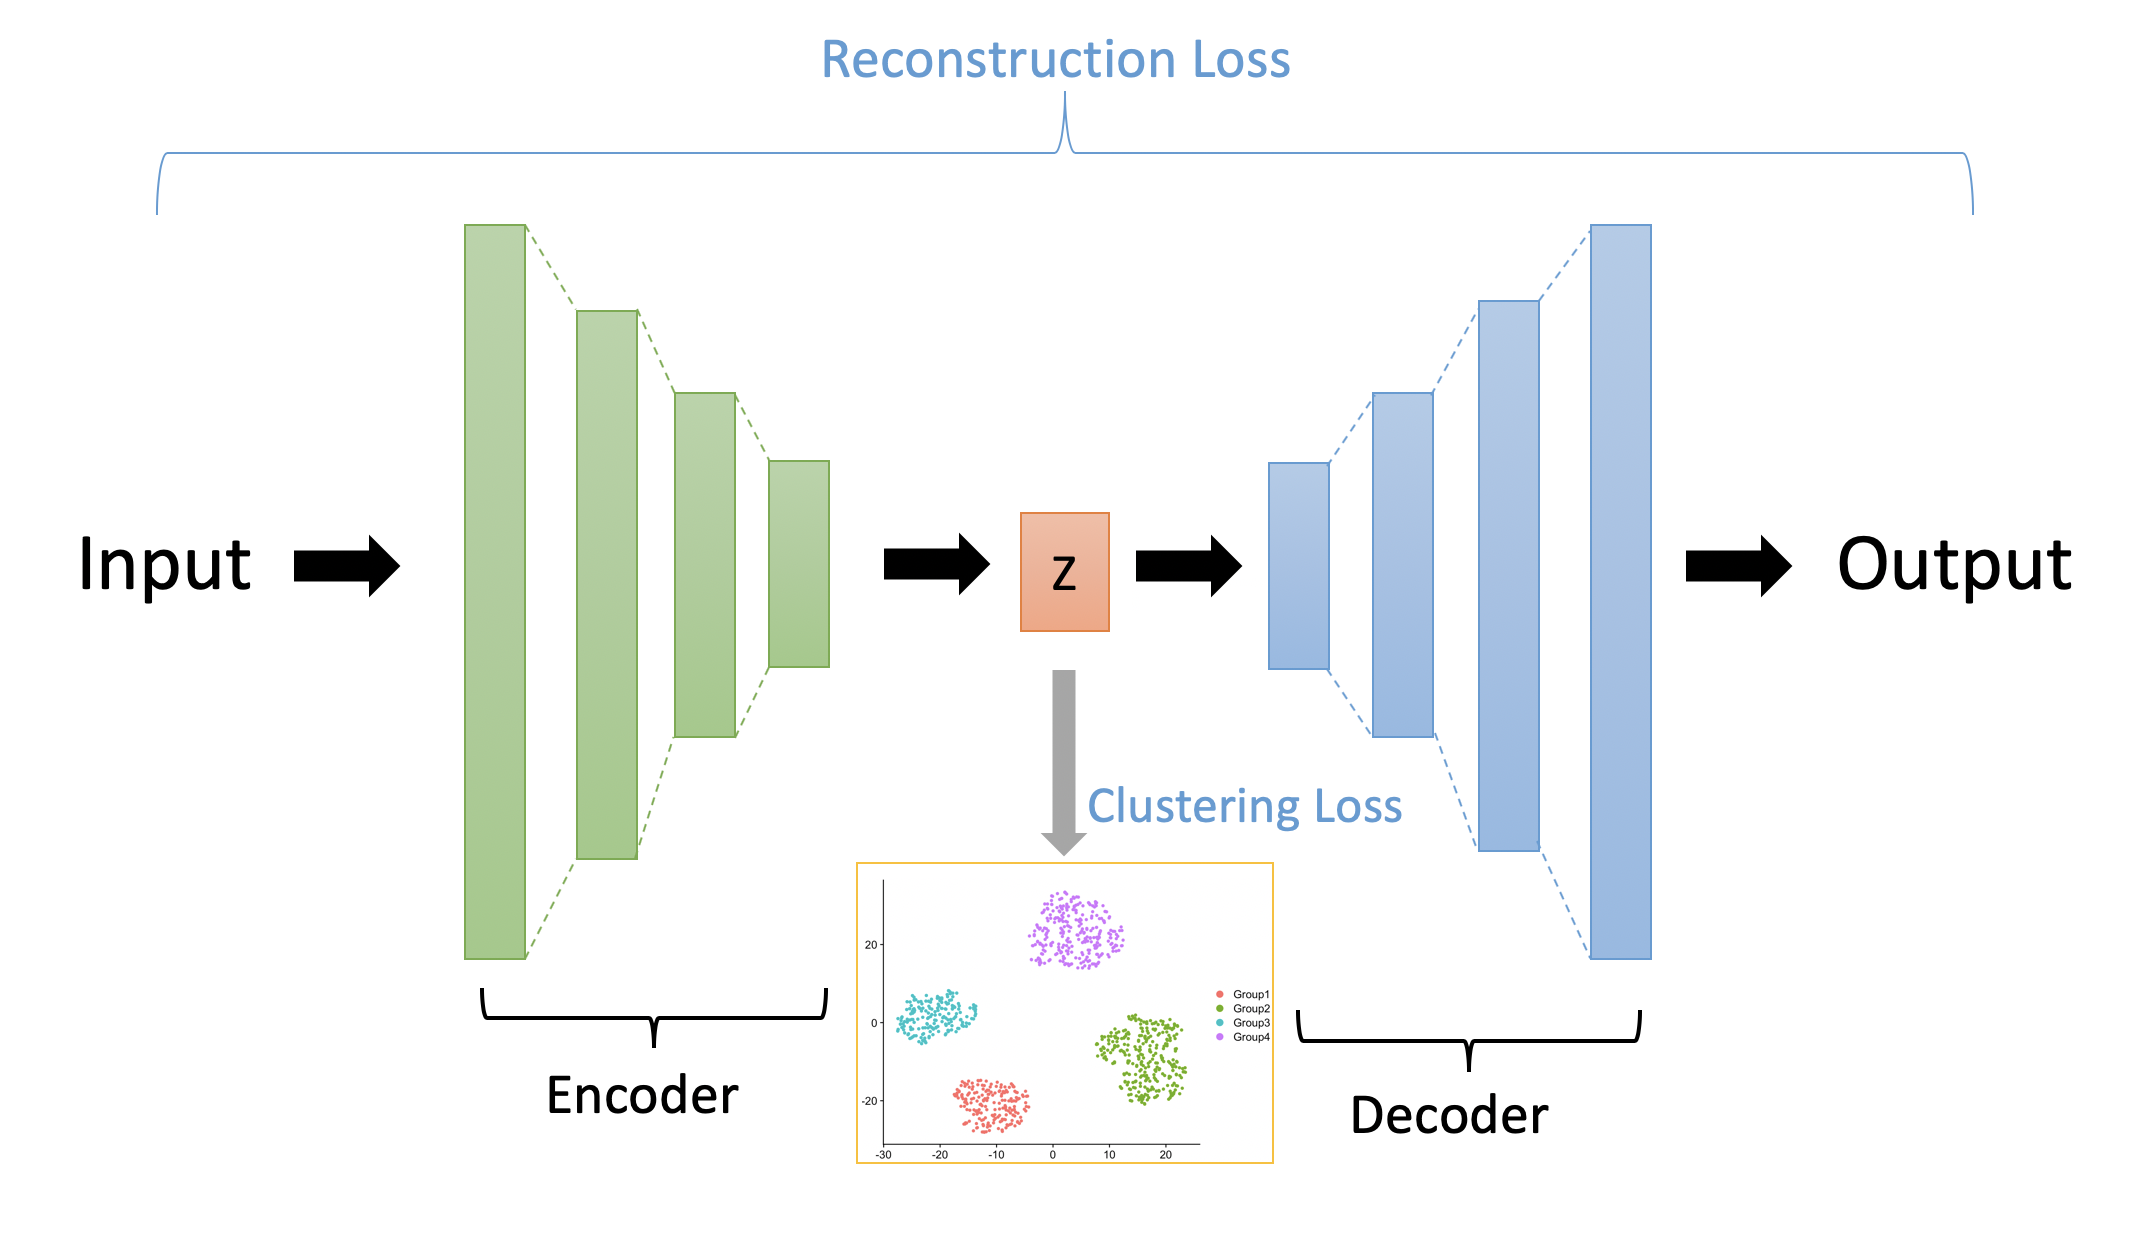
\includegraphics[width=1\textwidth]{figures/myfigures/dc.png}
    \caption{The structure of the deep clustering model}
    \label{dcstru}
\end{figure}

For the clustering process, we tried four methods: the spectral clustering \cite{von2007tutorial}, DBSCAN \cite{ester1996density}, K-means \cite{kanungo2002efficient} and louvain methods \cite{traag2019louvain}. 

The optimization of this model consists two parts. Firstly, pre-train the network as a normal variational autoencoder. Then, performing alternating trainging to optimize the clustering loss and reconstruction loss at the same time.

\subsection{GVAE for scRNA-seq data}
Recent years, with the development of deep learning, graph neuron network has been widely used in various industries such as social network \cite{yang2016revisiting}, recommendation systems \cite{kipf2016semi}. Single-cell sequencing data can also be viewed as a graph where each node is a cell. For example, a study \cite{ravindra2020disease} uses graph convolutional neuron network \cite{velivckovic2017graph} to predict the disease state of Multiple Sclerosis. The graph structure can also be applied to the variational autoencoder model \cite{kipf2016variational}. It is possible that though the preservation of graph structure of single cells in high dimensionality spaces, graph variational autoencoder can have better dimensionality reduction performance on global cell structures.



